\documentclass{article}

%%%%%%%%%%%%%%%%%%%%%%%%%%%%%%%%%%%%%%%%%%%%%%%%%%%%%%%%%%%%%%%%%
%package

%geometry
\usepackage[a4paper]{geometry}%调整页面边距
\geometry{left=3cm,right=3cm,top=3cm,bottom=3cm}
\linespread{1.5}
\usepackage{fancyhdr}%梦幻页眉

%fonts
\usepackage{fontspec}%字体库
\defaultfontfeatures{Mapping=tex-text}
\usepackage{xunicode,xltxtra}
\usepackage[BoldFont,SlantFont,CJKnumber,CJKchecksingle]{xeCJK}  % \CJKnumber{12345}: 一万二千三百四十五
\usepackage{CJKfntef}
\usepackage{bm} %公式中的粗体字符\boldsymbol
\usepackage{pifont}

%color
\usepackage{color,xcolor}
\definecolor{GREEN}{RGB}{25,180,68}
\definecolor{YELLOW}{RGB}{255,255,224}
\definecolor{BLUE}{RGB}{9,148,234}
\definecolor{RED}{RGB}{139,0,0}
\definecolor{DRED}{RGB}{128,0,0}
\definecolor{GREY}{RGB}{128,128,128}
\usepackage[pagecolor={YELLOW}]{pagecolor}%设置页面底色

%math
\usepackage{amsmath,amsfonts,amssymb}

%graphics
\usepackage[americaninductors,europeanresistors]{circuitikz}
\usepackage{tikz}%可以绘制各种坐标图,方格图
\usetikzlibrary{positioning,arrows,shadows,shapes,calc,mindmap,trees,backgrounds}  % placements=positioning
\usepackage{graphicx}%\includegraphics插图命令
\usepackage{subfigure}  %%图形或表格并排排列

% table
\usepackage{colortbl,dcolumn}  %% 彩色表格
\usepackage{multirow}
\usepackage{multicol}
\usepackage{booktabs}

% code
\usepackage{fancyvrb}%漂亮的代码包
\usepackage{listings}%加入代码

% ref
\usepackage{hyperref}%扩展参考文献,目录功能和加入超链接。

% title
\usepackage{titlesec}%花哨的章节标题

\usepackage{etoolbox}
\makeatletter
\patchcmd{\ttlh@hang}{\parindent\z@}{\parindent\z@\leavevmode}{}{}
\patchcmd{\ttlh@hang}{\noindent}{}{}{}
\makeatother%titlesec旧版本无编号问题


\titleformat
{\section} % command
[display] % shape
{\bfseries\Large} % format
{第\ \thesection 章\ } % label
{0.3ex} % sep
{
    \rule{\textwidth}{1pt}
    \vspace{1ex}
    \centering
} % before-code
[
\vspace{-2ex}%
\rule{\textwidth}{1pt}
] % after-code


%tightly-packed lists
\usepackage{mdwlist}
\usepackage{verbatim}%comment命令的注释包
\usepackage{styles/zhfontcfg}%中文包
\usepackage{styles/visionouclistings}
\usepackage{styles/visionouccfg}

% head/foot
\setlength{\headheight}{15pt}

\fancyhf{}



%%%%%%%%%%%%%%%%%%%%%%%%%%%%%%%%%%%%%%%%%%%%%%%%%%%%%%%%%%%%%%%%%%%%%%

%settings
\setCJKmainfont{Adobe Kaiti Std} %设置为楷体
\setCJKmonofont{Adobe Fangsong Std}%仿宋
%页眉页脚


\makeatletter
\def\headrule{{\if@fancyplain\let\headrulewidth\plainheadrulewidth\fi%
\hrule\@height 2.5pt \@width\headwidth\vskip1pt%上面线为2.5pt粗  
\hrule\@height 0.5pt\@width\headwidth  %下面0.5pt粗            
\vskip-2\headrulewidth\vskip-1pt}      %两条线的距离        
\vspace{6mm}}     %双线与下面正文之间的垂直间距              
\makeatother         
 

% graphics
\graphicspath{{figures/}}
\tikzset{
    % Define standard arrow tip
    >=stealth',
    % Define style for boxes
    punkt/.style={
           rectangle,
           rounded corners,
           draw=black, very thick,
           text width=6.5em,
           minimum height=2em,
           text centered},
    % Define arrow style
    pil/.style={
           ->,
           thick,
           shorten <=2pt,
           shorten >=2pt,},
    % Define style for FlyZhyBall
    FlyZhyBall/.style={
      circle,
      minimum size=6mm,
      inner sep=0.5pt,
      ball color=red!50!blue,
      text=white,},
    % Define style for FlyZhyRectangle
    FlyZhyRectangle/.style={
      rectangle,
      rounded corners,
      minimum size=6mm,
      ball color=red!50!blue,
      text=white,},
    % Define style for zhyfly
    zhyfly/.style={
      rectangle,
      rounded corners,
      minimum size=6mm,
      ball color=red!25!blue,
      text=white,},
    % Define style for new rectangle
    nrectangle/.style={
      rectangle,
      draw=#1!50,
      fill=#1!20,
      minimum size=5mm,
      inner sep=0.1pt,}
}

% code
\lstnewenvironment{VHDLcode}[1][]{%
  \lstset{
    basicstyle=\footnotesize\ttfamily\color{black},%
    columns=flexible,%
    framexleftmargin=.7mm,frame=shadowbox,%
    rulesepcolor=\color{blue},%
%    frame=single,%
    backgroundcolor=\color{yellow!20},%
    xleftmargin=1.2\fboxsep,%
    xrightmargin=.7\fboxsep,%
    numberstyle=\tiny\color{blue},%
    numberblanklines=false,numbersep=7pt,%
    language=VHDL%
    }\lstset{#1}}{}
\lstnewenvironment{VHDLmiddle}[1][]{%
  \lstset{
    basicstyle=\scriptsize\ttfamily\color{black},%
    columns=flexible,%
    framexleftmargin=.7mm,frame=shadowbox,%
    rulesepcolor=\color{blue},%
%    frame=single,%
    backgroundcolor=\color{yellow!20},%
    xleftmargin=1.2\fboxsep,%
    xrightmargin=.7\fboxsep,%
    numbers=left,numberstyle=\tiny\color{blue},%
    numberblanklines=false,numbersep=7pt,%
    language=VHDL%
    }\lstset{#1}}{}
\lstnewenvironment{VHDLsmall}[1][]{%
  \lstset{
    basicstyle=\tiny\ttfamily\color{black},%
    columns=flexible,%
    framexleftmargin=.7mm,frame=shadowbox,%
    rulesepcolor=\color{blue},%
%    frame=single,%
    backgroundcolor=\color{yellow!20},%
    xleftmargin=1.2\fboxsep,%
    xrightmargin=.7\fboxsep,%
    numbers=left,numberstyle=\tiny\color{blue},%
    numberblanklines=false,numbersep=7pt,%
    language=VHDL%
    }\lstset{#1}}{}
% pdf
\hypersetup{pdfauthor={Haiyong Zheng},%
            pdftitle={Title},%
            CJKbookmarks=true,%
            bookmarksnumbered=true,%
            bookmarksopen=false,%
            plainpages=false,%
            colorlinks=true,%
            citecolor=green,%
            filecolor=magenta,%
            linkcolor=DRED,%red(default)
            urlcolor=cyan}
\newcommand\titlebar{%
\tikz[baseline,trim left=3.1cm,trim right=3cm] {
    \fill [cyan!25] (2.5cm,-1ex) rectangle (\textwidth+3.1cm,2.5ex);
    \node [
        fill=cyan!60!white,
        anchor= base east,
        rounded rectangle,
        minimum height=3.5ex] at (3cm,0) {
        \textbf{\thesection.}
    };
}%
}

%code
\definecolor{mygreen}{rgb}{0,0.6,0}
\definecolor{mygray}{rgb}{0.5,0.5,0.5}
\definecolor{mymauve}{rgb}{0.58,0,0.82}
\lstset{
 backgroundcolor=\color{white}, 
 basicstyle = \footnotesize,       
 breakatwhitespace = false,        
 breaklines = true,                 
 captionpos = b,                    
 commentstyle = \color{mygreen}\bfseries,
 extendedchars = false,             
 frame =shadowbox, 
 framerule=0.5pt,
 keepspaces=true,
 keywordstyle=\color{blue}\bfseries, % keyword style
 language = C++,                     % the language of code
 otherkeywords={string}, 
 numbers=left, 
 numbersep=5pt,
 numberstyle=\tiny\color{mygray},
 rulecolor=\color{black},         
 showspaces=false,  
 showstringspaces=false, 
 showtabs=false,    
 stepnumber=1,         
 stringstyle=\color{mymauve},        % string literal style
 tabsize=2,          
 title=\lstname                      
}


%%%%%%%%%%%%%%%%%%%%%%%%%%%%%%%%%%%%%%%%%%%%%%%%%%%%%%%%%%%
%设置标题页面

\newcommand*{\titleGM}{\begingroup % 新命令:添加标题页
\hbox{ % 水平盒子
\hspace*{0.2\textwidth} % 左边空白
\rule{1pt}{\textheight\color{GREY}} % 竖线
\hspace*{0.05\textwidth} % 竖线和文本距离
\parbox[b]{0.75\textwidth}{ % 文本最大右边距

{\noindent\Huge\bfseries 图像内插 \\[0.5\baselineskip] Image Interpolation}\\[2\baselineskip] % 题目
{\large \textit{三种传统内插方法介绍与解析}}\\[4\baselineskip] % 标签或描述
{\Large \textsc{丁昊}}\\ % 作者

\vspace{0.5\textheight} % 题目区域和作者间距
{\noindent August 2016 }\\[\baselineskip] % Publisher and logo
}}
\endgroup}


                      
\chead{\color{GREY}IMAGE INTERPOLATION}%页眉
\cfoot{\color{GREY}August 2016}%页脚 中
\lfoot{\color{GREY}DingHao}%页脚 左
\rfoot{\color{GREY}$\cdot$\ Page \thepage\ }%页脚 右
\renewcommand{\headrulewidth}{0.4pt}
\renewcommand{\footrulewidth}{0.4pt}

\usepackage{styles/lshort}

%%%%%%%%%%%%%%%%%%%%%%%%%%%%%%%%%%%%%%%%%%%%%%%%%%%%%%%%%%%%%%%%%
\begin{document}


\titleGM\thispagestyle{empty}

\pagenumbering{roman}

\setcounter{page}{0}
\newpage

\begin{abstract}

内插是在诸如放大、收缩、旋转和几何校正等任务中广泛应用的基本工具。放大图像(或称为上采样(upsampling)或图像插值(interpolating))的主要目的是放大原图像,从而可以显示在更高分辨率的显示设备上。图像放大几乎都是采用内插值方法,即在原有图像像素的基础上在像素点之间采用合适的插值算法插入新的元素。

\end{abstract}
\newpage

\tableofcontents 
\newpage

\pagestyle{fancy}

\pagenumbering{arabic}
\newpage
%%%%%%%%%%%%%%%%%%%%%%%%%%%%%%%%%%%%%%%%%%%%%%%%%%%%%%%%%%%%%%%%%

\section{基本概念}

内插是一个通过已知的离散数据求未知数据的过程,我所研究的这一部分是利用内插方法来放大一个图像。

对于一副原图像,假设我们想将它放大到原来大小的2倍,那么设想一下,因为每个像素点的大小是相同的,在长和宽变为两倍后,像素点的个数自然变为了原来的4倍。如果我们想使放大后的图像尽量的不失真,就需要通过某种方法,根据原图仅有的像素点来求得放大后图像中每个像素点的值。这个过程就是内插。

拿最近邻内插来解释说明。我们先预设一个原来两倍大小的图像,将其等比例对应到原图的每个像素点。当然,因为新图像素点的个数为原图的四倍,所以对应的相同位置上原图的一个像素点就对应了新图的四个像素点。这时,使新图的每个像素点都等于原图对应位置的像素值,就完成了最近邻内插过程。我举得这个例子是正好成倍数的,绝大部分情况并非这样,但原理相同,即将对应位置最近邻的一个点的值赋给新图。
\newpage

\section{分类}


\begin{itemize}

\item 传统插值:最近邻内插,双线性内插,三线性内插。也是DIP课本上介绍的三类内插。
\item 给予边缘的图像插值算法:基于原始低分辨图像边缘的方法和基于插值后高分辨率图像边缘的方法。基于原始低分辨率图像边缘的方法:
首先检测低分辨率图像的边缘, 然后根据检测的边缘将像素分类处理, 对于平坦区域的像素,采用传统方法插值;对于边缘区域的像素, 设计特殊插值方法, 以达到保持边缘细节的目的。
基于插值后高分辨率图像边缘的方法这类插值方法:首先采用传统方法插值低分辨率图像,然后检测高分辨率图像的边缘,最后对边缘及附近像素进行特殊处理, 以去除模糊, 增强图像的边缘。
\item 给予区域的图像插值算法:首先将原始低分辨率图像分割成不同区域,然后将插值点映射到低分辨率图像, 判断其所属区域, 最后根据插值点的邻域像素设计不同的插值公式, 计算插值点的值。
\item 偏微分方程插值(PDE),分形,小波逆向插值这三种也是插值算法的主流之一。小波与分形算法计算复杂度高,效果较好,小波边缘处理最好,分形次之。

\end{itemize}
\newpage

\section{最近邻内插}

最近邻内插即在基本概念中所解释的过程,取的是对应点最近邻的值。

\subsection{代码}

\begin{lstlisting}[caption={}]

#include <iostream> 
#include <opencv2/imgproc/imgproc.hpp>
#include <opencv2/highgui/highgui.hpp>
#include <math.h>

using namespace cv;
using namespace std;

    int main(int argc, char* argv[])  
    {
	//放大倍数  
	double x=2;

        //读图语句报错
	if ( argc != 2 )
	{
		cout<<"Wrong arguments."<<endl;
		cout<<"Usage:"<<endl;
		cout<<"\t "<<argv[0]<<" Image"<<endl;
		exit(7);
	}

	string image = argv[1];
        Mat src = imread(image);  
       
	//读图格式报错
	if( !src.data )
	{
		cout<<"Can't process this kind of image"<<endl;
		exit(8);
	}

        //显示  
        imshow("src",src);  
      
        //处理长宽  
	int row=src.rows;
	int col=src.cols;
	float nrow=x*(float)row;
	float ncol=x*(float)col;
	
	//创建矩阵
        Mat dst = Mat::zeros(nrow,ncol,CV_8UC3);  
      	int X=0;
	int Y=0;

	//最邻近内插
	for ( int i = 0; i < nrow; i++)
	{
		for(int j = 0; j < ncol; j++)
		{
			X= cvRound ( i / (double)x );
			Y= cvRound ( j / (double)x );
			if( X < row && X >= 0 && Y >= 0 && Y <= col )
			{	
				dst.at<cv::Vec3b>(i,j)[0]=src.at<cv::Vec3b>(X,Y)[0];
				dst.at<cv::Vec3b>(i,j)[1]=src.at<cv::Vec3b>(X,Y)[1];
				dst.at<cv::Vec3b>(i,j)[2]=src.at<cv::Vec3b>(X,Y)[2];
			}
		}
	}        


      
        imshow("dst",dst);  
 	imwrite("nearest.bmp",dst);
        waitKey(0);  
        return 0;  
    }  

\end{lstlisting}

\newpage
\subsection{结果}

\begin{figure}[htbp]

  \centering

\subfigure[原图]{\label{fig:fft:a}

\begin{minipage}[c]{0.5\textwidth}

\centering

  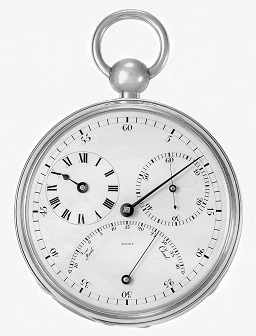
\includegraphics[width=5.5cm]{1.jpg}

\end{minipage}%

}%注意这个”%”绝对不能省,可以试试不打%的效果

\subfigure[效果图]{

\begin{minipage}[c]{0.5\textwidth}

\centering

  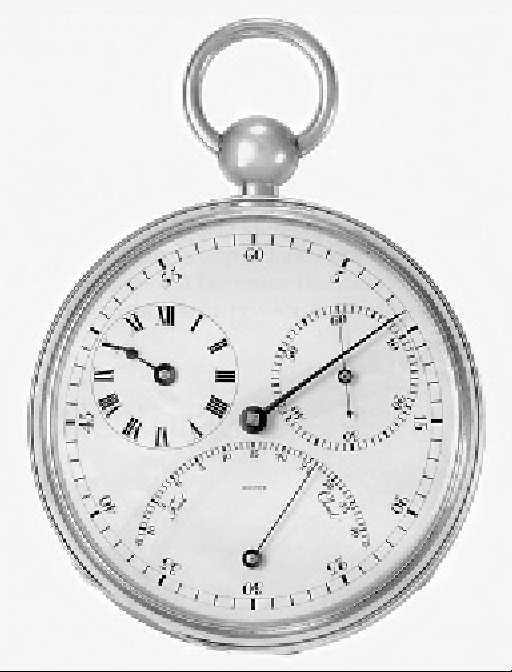
\includegraphics[width=5.5cm]{nearest.jpg}

\end{minipage}

}

\caption{最近邻内插}\label{fig:fft}

\end{figure}
\newpage

\section{双线性内插}

\subsection{原理}
双线性内插的赋值由下面公式得到:

$f(x,y) \approx f(0,0)(1-x)(1-y)+f(1,0)x(1-y)+f(0,1)(1-x)y+f(1,1)xy$

其中f(0,0)、f(1,0)、f(0,1)、f(1,1)四个点为目标图像像素点对应到原图的四个最近邻点,x、y的值并非绝对坐标而是相对坐标,即0到1之间的小数。
将上式化简即可得到书上的公式:

\begin{math}
v(x,y)=ax+by+cxy+d
\end{math}

而四个系数的取值此时为:
\begin{itemize}
\item a=f(1,0)-f(0,0)
\item b=f(0,1)-f(0,0)
\item c=f(1,1)-f(0,1)-f(1,0)+f(0,0)
\item d=f(0,0)
\end{itemize}
然而,用这种取系数的方法会导致输出图像部分溢出,所以不推荐使用。
\newpage
\subsection{代码}

\begin{lstlisting}

#include <iostream> 
#include <opencv2/imgproc/imgproc.hpp>
#include <opencv2/highgui/highgui.hpp>
#include <math.h>

using namespace cv;
using namespace std;

    int main(int argc, char* argv[])  
    {
	//放大倍数  
	double x=2;

        //读图语句报错
	if ( argc != 2 )
	{
		cout<<"Wrong arguments."<<endl;
		cout<<"Usage:"<<endl;
		cout<<"\t "<<argv[0]<<" Image"<<endl;
		exit(7);
	}

	string image = argv[1];
        Mat src = imread(image);  
       
	//读图格式报错
	if( !src.data )
	{
		cout<<"Can't process this kind of image"<<endl;
		exit(8);
	}

        //显示  
        imshow("src",src);  
      
        //处理长宽  
	int row=src.rows;
	int col=src.cols;
	float nrow=x*(float)row;
	float ncol=x*(float)col;
	
	//创建矩阵
        Mat dst = Mat::zeros(nrow,ncol,CV_8UC3);  
      	
	float X=0,Y=0;
	CvScalar a,b,c,d;

	//双线性内插
	for ( int i = 0; i < nrow-1; i++)
	{
		for(int j = 0; j < ncol-1; j++)
		{
			X= i / (double)x ;
			Y= j / (double)x ;
			float ux=(int)X,uy=(int)Y;
			ux=abs(ux-X);uy=abs(uy-Y);
			
			if( X < row-1 && X >= 0 && Y >= 0 && Y < col-1 )
			{
		//取四个点
			a = src.at<cv::Vec3b>((int)X,(int)Y);
			b = src.at<cv::Vec3b>((int)X,(int)Y+1);
			c = src.at<cv::Vec3b>((int)X+1,(int)Y);
			d = src.at<cv::Vec3b>((int)X+1,(int)Y+1);
			}
		//系数相加为处理后的点值
				dst.at<cv::Vec3b>(i,j)[0]=(a.val[0]*(1-ux)+c.val[0]*ux)*(1-uy)+(b.val[0]*(1-ux)+d.val[0]*ux)*uy;
				dst.at<cv::Vec3b>(i,j)[1]=(a.val[1]*(1-ux)+c.val[1]*ux)*(1-uy)+(b.val[1]*(1-ux)+d.val[1]*ux)*uy;
				dst.at<cv::Vec3b>(i,j)[2]=(a.val[2]*(1-ux)+c.val[2]*ux)*(1-uy)+(b.val[2]*(1-ux)+d.val[2]*ux)*uy;
			
		}
	}        


      
        imshow("dst",dst);  
      	imwrite("double.bmp",dst);

        waitKey(0);  
        return 0;  
    }  

\end{lstlisting}

\newpage
\subsection{结果}

\begin{figure}[htbp]

  \centering

\subfigure[原图]{\label{fig:fft:a}

\begin{minipage}[c]{0.5\textwidth}

\centering

  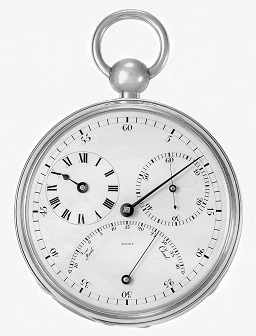
\includegraphics[width=5.5cm]{1.jpg}

\end{minipage}%

}%注意这个”%”绝对不能省,可以试试不打%的效果

\subfigure[效果图]{

\begin{minipage}[c]{0.5\textwidth}

\centering

  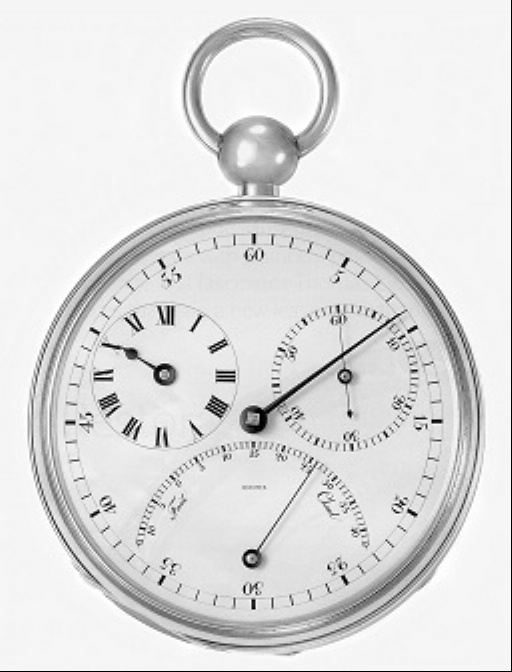
\includegraphics[width=5.5cm]{Bilinear-pots.jpg}

\end{minipage}

}

\caption{双线性内插}\label{fig:fft}

\end{figure}
\newpage

\section{双三次内插}

\subsection{原理}
双三次插值通过下式进行计算:

$f(x,y)=a_{00}+a_{10}x+a_{01}y+a_{20}x^{2}+a_{11}xy+a_{02}y^{2}+a_{21}x^{2}y+a_{12}xy^{2}+a_{22}x^{2}y^{2}+a_{30}x^{3}+a_{03}y^{3}+a_{31}xy^{3}+a_{32}x^{3}y^{2}+a_{23}x^{2}y^{3}+a_{33}x^{3}y^{3}$

也就是:

$f(x,y)=\sum _{i=0}^{3}\sum _{j=0}^{3}a_{ij}x^{i}y^{j}$

计算系数 $a_{ij}$ 的取值依赖于插值数据的特性。如果已知插值函数的导数,常用的方法就是使用四个顶点的高度以及每个顶点的三个导数。一阶导数$h'x$与$h'y$ 表示x、y放心的表面斜率,二阶相互导数$h''xy$表示同时在x与y方向的斜率。这些值可以通过分别连续对x与y向量取微分得到。对于网格单元的每个顶点,将局部坐标(0,0)、(1,0)、(0,1)和(1,1)带入这些方程,再解这16个方程。

\newpage
\subsection{代码}

\begin{lstlisting}
#include <iostream> 
#include <opencv2/imgproc/imgproc.hpp>
#include <opencv2/highgui/highgui.hpp>
#include <math.h>

using namespace cv;
using namespace std;

int main(int argc, char* argv[])  
    {  
        //导入图像
	if ( argc != 2 )
	{
		cout<<"Wrong arguments."<<endl;
		cout<<"Usage:"<<endl;
		cout<<"\t "<<argv[0]<<" Image"<<endl;
		exit(7);
	}


	string image = argv[1];
        Mat src = imread(image);  

      //读图格式报错
	if( !src.data )
	{
		cout<<"Can't process this kind of image"<<endl;
		exit(8);
	}

        //显示  
        imshow("src",src);  
      
	Mat dst;
	resize(src,dst,Size(),2,2,INTER_CUBIC);        

      
        imshow("dst",dst);  
     	imwrite("nearest-resize.bmp",dst); 
        waitKey(0);  
        return 0;  
    }  
\end{lstlisting}
\newpage
\subsection{结果}

\begin{figure}[htbp]

  \centering

\subfigure[原图]{\label{fig:fft:a}

\begin{minipage}[c]{0.5\textwidth}

\centering

  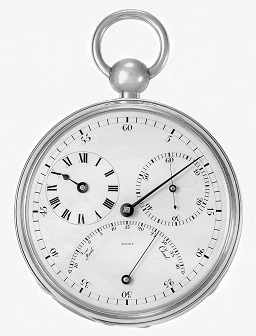
\includegraphics[width=5.5cm]{1.jpg}

\end{minipage}%

}%注意这个”%”绝对不能省,可以试试不打%的效果

\subfigure[效果图]{

\begin{minipage}[c]{0.5\textwidth}

\centering

  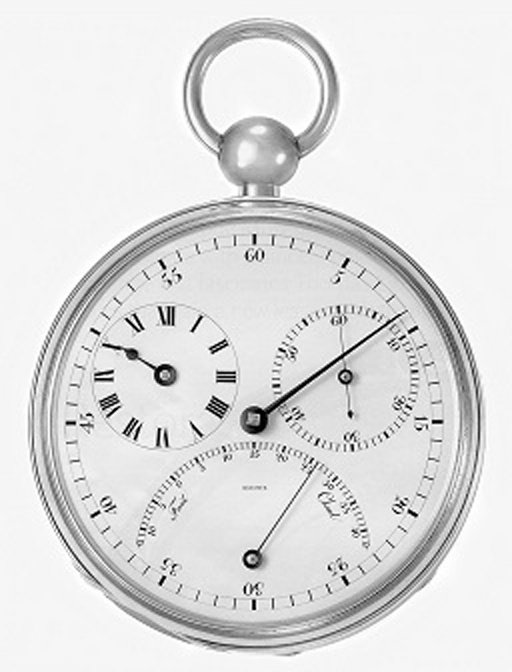
\includegraphics[width=5.5cm]{Bicubic.jpg}

\end{minipage}

}

\caption{双三次内插}\label{fig:fft}

\end{figure}

\end{document}
